\documentclass[12pt,a4paper,twoside,sumario=abnt-6027-2012,chapter=TITLE]{abntex2}
%%%%%%%%%%%%%%%%%%%%%%%%%%%%%%%%%%%%%%%%%%%%%%%%%%%%%%%%%%%%%%%%%%%%%%
%% Esse arquivo inclui os pacotes e configurações utilizados
%% para adequar o modelo.
%%
%%  **** Não é necessário modificar esse arquivo ****
%%
%%%%%%%%%%%%%%%%%%%%%%%%%%%%%%%%%%%%%%%%%%%%%%%%%%%%%%%%%%%%%%%%%%%%%%

\usepackage{scrextend} % para usar o ambiente labeling
\usepackage{array}
\usepackage{scalefnt} %escala de tabelas
\usepackage[brazil]{babel}
\usepackage{mathptmx} %Times new roman para texto e matemática
%\usepackage{times}   %Times new roman para texto
\usepackage{lastpage}
\usepackage{minitoc} 
\usepackage[utf8]{inputenc}
\usepackage{amsmath}
\usepackage{amsfonts}
\usepackage{amssymb}
\usepackage{graphicx}	
\usepackage[]{pdfpages} %permite colocar pdf no texto

\sloppy

%%==================================================================
%% INÍCIO
%% Permite colocar código (Algoritmos) 
%% https://pt.overleaf.com/learn/latex/Code_listing
%%==================================================================
\usepackage{listings} 
\usepackage{xcolor}

%% As linhas abaixo permitem várias personalizações
\definecolor{codegreen}{rgb}{0,0.6,0}
\definecolor{codegray}{rgb}{0.5,0.5,0.5}
\definecolor{codepurple}{rgb}{0.58,0,0.82}
\definecolor{backcolour}{rgb}{0.95,0.95,0.92}
 
\lstdefinestyle{mystyle}{
    backgroundcolor=\color{backcolour},   
    commentstyle=\color{codegreen},
    keywordstyle=\color{magenta},
    numberstyle=\tiny\color{codegray},
    stringstyle=\color{codepurple},
    basicstyle=\ttfamily\footnotesize,
    breakatwhitespace=false,         
    breaklines=true,                 
    captionpos=b,                    
    keepspaces=true,                 
    numbers=left,                    
    numbersep=5pt,                  
    showspaces=false,                
    showstringspaces=false,
    showtabs=false,                  
    tabsize=2
}
 
\lstset{style=mystyle}
%%==================================================================
%% FIM
%% Permite colocar código (Algoritmos) 
%%==================================================================


%%==================================================================
%% INÍCIO
%% Configurações de espaçamento entre títulos dos capítulos e seções
%%==================================================================
% Coloca o espaçamento 1,5 entre títulos de capítulos e o texto. 
% Coloca tanto antes quanto depois. Norma abnt e manual da UFVJM
\setlength\afterchapskip{\lineskip} 
\setlength\beforechapskip{\lineskip}
%coloca o espaçamento 1,5 entre títulos de seções e o texto. 
%Coloca tanto antes quanto depois. Norma abnt e manual da UFVJM
\setlength\aftersecskip{\lineskip}
\setlength\beforesecskip{\lineskip}
%Coloca o espaçamento 1,5 entre títulos de subseções e o texto. 
%Coloca tanto antes quanto depois. Norma abnt e manual da UFVJM
\setlength\aftersubsecskip{\lineskip}
\setlength\beforesubsecskip{\lineskip}
% Coloca o espaçamento 1,5 entre títulos de subsubseções e o texto. 
% Coloca tanto antes quanto depois. Norma abnt e manual da UFVJM
\setlength\aftersubsubsecskip{\lineskip}
\setlength\beforesubsubsecskip{\lineskip}
%%==================================================================
%% FIM 
%% Configurações de espaçamento entre títulos dos capítulos e seções
%%==================================================================

%%==================================================================
%% INÍCIO
%% Euler - pacotes para múltiplas linhas e colunas de tabelas
%%==================================================================
\usepackage{multirow}
\usepackage{multicol}
%%==================================================================
%% FIM 
%% Euler - pacotes para múltiplas linhas e colunas de tabelas
%%==================================================================



%%%marcelo - Caption do tipo do elemento gráfico em negrito.

%\usepackage[labelfont=bf]{caption}

%%% Ex: Figura 1 - Título da figura.
%%% Apenas Figura 1 estará em negrito

%%%marcelo - Todo caption em negrido

\usepackage{caption}
% marcelo - colocar a fonte alinhada a esquerda
%https://tex.stackexchange.com/questions/131532/position-caption-of-centered--left-adjusted-to-figure
%\captionsetup{font={bf,small}, position=below, justification=raggedright, singlelinecheck=false} % negrito e menor
\captionsetup{font={bf,small}, position=below,labelsep=endash} % negrito e menor
%%% tamanhos disponíveis -> scriptsize, footnotesize, small, normalsize, large, Large

%%% Ex: Figura 1 - Título da figura
%%% Figura 1 - Título da figura estará em negrito.
%% Euler: para colocar o travessão: labelsep=endash
% marcelo - Deixa a fonte da figura, quadro, etc, sem negrito quando se utiliza a solução acima.
%\newcommand{\fonteUFVJM}[1]{\legend{\textnormal{Fonte -- #1}}}
\renewcommand{\fonte}[1]{\captionsetup{justification=raggedright, singlelinecheck=false}\legend{\textnormal{Fonte: #1}}}

%\renewcommand{\fonte}[1]{\legend{\textnormal{Fonte: #1}}}


% marcelo - simula aspas duplas no estilo usado pelo JSON (''a'')
\newcommand{\q}[1]{{\textquotesingle\textquotesingle}#1{\textquotesingle\textquotesingle}}
%marcelo - nome menor para backslash
\newcommand{\bks}{\textbackslash}

\usepackage{tabularx} % marcelo - tabelas justificadas
\usepackage{booktabs} % marcelo - grossura da linha em tabelas

%%% marcelo - retira espaços extras entre os elementos de uma lista (itemize e enumarate)
\usepackage{enumitem}
\usepackage{setspace}
\setlist[itemize,enumerate]{nosep} % Caso queira deixar espaçamento duplo entre o parágravo anterior e posterior, mas não entre itens da lista, utilizar noitemsep no lugar de nosep
%%% até aqui

\raggedbottom % marcelo - Resolve o problema do espaçamento entre parágrafos aleatório

\usepackage{subfig} %marcelo - Suporte a subfiguras	

%\usepackage[none]{hyphenat} %marcelo - não permite hifenização


\usepackage{indentfirst}		
\usepackage{color}				
\usepackage{microtype}
%\usepackage[alf,abnt-emphasize=bf]{abntex2cite}

%resolve problemas com as referências
%% Versão justificada das referências
%\usepackage[alf,abnt-etal-cite=3,abnt-etal-list=0,abnt-etal-text=emph,abnt-emphasize=bf]{abntex2cite}

%% Versão alinhada à esquerda das referências
\usepackage[alf,abnt-etal-cite=3,abnt-etal-list=0,abnt-etal-text=emph,abnt-emphasize=bf]{abntex2cite}

\usepackage{ragged2e} %para usar o comando \justify
\usepackage{enumitem} %para mudar as alíneas
\usepackage{textcomp} %fornece caracteres especiais
\setlength{\parindent}{2cm} %Tamanho do parágrafo
%\setlength{\parskip}{1.5cm} 
%\setlrmarginsandblock{3cm}{2cm}


%Para definir o tamanho das fontes das seções, subseções, etc (+++ seria o item (subsection, section, chapter, etc):

\renewcommand{\ABNTEXchapterfontsize}{\normalsize} 
\renewcommand{\ABNTEXsectionfontsize}{\normalsize} 
\renewcommand{\ABNTEXsubsectionfontsize}{\normalsize} 
\renewcommand{\ABNTEXsubsubsectionfontsize}{\normalsize}

%Para deixar as fontes das seções, subseções, etc, em negrito (+++ seria o item (subsection, section, chapter, etc):

\renewcommand{\ABNTEXchapterfont}{\normalfont\normalfont\bfseries}
\renewcommand{\ABNTEXsectionfont}{\normalfont\bfseries}
\renewcommand{\ABNTEXsubsectionfont}{\normalfont\itshape\bfseries}
\renewcommand{\ABNTEXsubsubsectionfont}{\normalfont\itshape}


%Alterar o tipo da fonte no sumário - MARCELO

% Secao secundaria (Section) Caixa baixa, Negrito, tamanho 12
%\renewcommand{\cftsectionfont}{\bfseries} %ponha \rmfamily se quiser serifadas...

% Secao terciaria (Subsection) Caixa baixa e italico no sumário
\renewcommand{\cftsubsectionfont}{\normalfont\itshape\bfseries}

% Secao quaternaria (Subsubsection) Caixa baixa, Negrito, sublinhado, tamanho 12
\renewcommand{\cftsubsubsectionfont}{\normalfont\itshape}

% Seção quinaria (subsubsubsection) Caixa baixa, sem negrito, tamanho 12
%\renewcommand{\cftparagraphfont}{\normalfont}

% MARCELO - Evitar linhas órfãs e viúvas
\widowpenalty=10000
\clubpenalty=10000



%%%%% Euler - Cria comando para citar fontes de figuras e tabelas.

\newcommand{\citefonte}[1]
{\citeauthor{#1}, \citeyear{#1}}


\hypersetup{
     	pagebackref=true,
		pdftitle={\@title}, 
		pdfauthor={\@author},
    	pdfsubject={\imprimirpreambulo},
	    pdfcreator={Nome do Aluno},
		pdfkeywords={abnt}{latex}{abntex}{abntex2}{trabalho acadêmico}, 
		colorlinks=true,       		
    	linkcolor=black,          	
    	citecolor=black,        	
    	filecolor=magenta,      		
		urlcolor=blue,
		bookmarksdepth=4
}

%%==================================================================
%% INÍCIO 
%% João Paulo / Felipe Túlio (PPGEd)
%% Mapas Gráficos ...
%%==================================================================

%% QUADROS
\newcommand{\quadroname}{Quadro}
\newcommand{\listofquadrosname}{Lista de quadros}
\newfloat[chapter]{quadro}{loq}{\quadroname}
\newlistof{listofquadros}{loq}{\listofquadrosname}
\newlistentry{quadro}{loq}{0}
% configurações para atender às regras da ABNT
\setfloatadjustment{quadro}{\centering}
\counterwithout{quadro}{chapter}
\renewcommand{\cftquadroname}{\quadroname\space} 
\renewcommand*{\cftquadroaftersnum}{\hfill--\hfill}
% Configuração de posicionamento padrão:
\setfloatlocations{quadro}{hbtp}

%% Mapas
\newcommand{\mapaname}{Mapa}
\newcommand{\listofmapasname}{}
\newfloat[chapter]{mapa}{lom}{\mapaname}
\newlistof{listofmapas}{lom}{\listofmapasname}
\newlistentry{mapa}{lom}{0}
\setfloatadjustment{mapa}{\centering}
\counterwithout{mapa}{chapter}
\renewcommand{\cftmapaname}{\mapaname\space} 
\renewcommand*{\cftmapaaftersnum}{\hfill--\hfill}
\setfloatlocations{mapa}{hbtp}

%% Graficos
\newcommand{\graficoname}{Gráfico}
\newcommand{\listofgraficosname}{}
\newfloat[chapter]{grafico}{logrf}{\graficoname}
\newlistof{listofgraficos}{logrf}{\listofgraficosname}
\newlistentry{grafico}{logrf}{0}
\setfloatadjustment{grafico}{\centering}
\counterwithout{grafico}{chapter}
\renewcommand{\cftgraficoname}{\graficoname\space} 
\renewcommand*{\cftgraficoaftersnum}{\hfill--\hfill}
\setfloatlocations{grafico}{hbtp}

%% Algoritmo
\newcommand{\algoritmoname}{Algoritmo}
\newcommand{\listofalgoritmosname}{Lista de Ilustrações} % Gambiarra 
\newfloat[chapter]{algoritmo}{loalg}{\algoritmoname}
\newlistof{listofalgoritmos}{loalg}{\listofalgoritmosname}
\newlistentry{algoritmo}{loalg}{0}
\setfloatadjustment{algoritmo}{\centering}
\counterwithout{algoritmo}{chapter}
\renewcommand{\cftalgoritmoname}{\algoritmoname\space} 
\renewcommand*{\cftalgoritmoaftersnum}{\hfill--\hfill}
\setfloatlocations{algoritmo}{hbtp}

% Gambiarra 
\addto\captionsbrazil{%
  \renewcommand{\listfigurename}%
    {}%
}

%%==================================================================
%% FIM 
%% João Paulo / Felipe (PPGEd)
%% Mapas Gráficos ...
%%==================================================================




%%==================================================================
%% INÍCIO 
%% Alexandre - Comandos adicionais 
%%==================================================================

% Comando para definir curso/programa
\providecommand{\imprimircurso}{}
\newcommand{\curso}[1]{\renewcommand{\imprimircurso}{#1}}

% Comando para Titulação do Orientador
\providecommand{\imprimirTitulacaoOrientador}{}
\newcommand{\TitulacaoOrientador}[1]{\renewcommand{\imprimirTitulacaoOrientador}{#1}}

% Comando para Titulação do Orientador
\providecommand{\imprimirDepartamentoOrientador}{}
\newcommand{\DepartamentoOrientador}[1]{\renewcommand{\imprimirDepartamentoOrientador}{#1}}

% Comando para Titulação do Coorientador
\providecommand{\imprimirTitulacaoCoorientador}{}
\newcommand{\TitulacaoCoorientador}[1]{\renewcommand{\imprimirTitulacaoCoorientador}{#1}}

% Comando para Titulação do Orientador
\providecommand{\imprimirDepartamentoCoorientador}{}
\newcommand{\DepartamentoCoorientador}[1]{\renewcommand{\imprimirDepartamentoCoorientador}{#1}}

%Membos da banca 
\providecommand{\imprimirMembroA}{}
\newcommand{\membroA}[1]{\renewcommand{\imprimirMembroA}{#1}}
\providecommand{\imprimirMembroB}{}
\newcommand{\membroB}[1]{\renewcommand{\imprimirMembroB}{#1}}
\providecommand{\imprimirMembroC}{}
\newcommand{\membroC}[1]{\renewcommand{\imprimirMembroC}{#1}}
\providecommand{\imprimirMembroD}{}
\newcommand{\membroD}[1]{\renewcommand{\imprimirMembroD}{#1}}
\providecommand{\imprimirTitulacaoMembroA}{}
\newcommand{\TitulacaoMembroA}[1]{\renewcommand{\imprimirTitulacaoMembroA}{#1}}
\providecommand{\imprimirTitulacaoMembroB}{}
\newcommand{\TitulacaoMembroB}[1]{\renewcommand{\imprimirTitulacaoMembroB}{#1}}
\providecommand{\imprimirTitulacaoMembroC}{}
\newcommand{\TitulacaoMembroC}[1]{\renewcommand{\imprimirTitulacaoMembroC}{#1}}
\providecommand{\imprimirTitulacaoMembroD}{}
\newcommand{\TitulacaoMembroD}[1]{\renewcommand{\imprimirTitulacaoMembroD}{#1}}
\providecommand{\imprimirDepartamentoMembroA}{}
\newcommand{\DepartamentoMembroA}[1]{\renewcommand{\imprimirDepartamentoMembroA}{#1}}
\providecommand{\imprimirDepartamentoMembroB}{}
\newcommand{\DepartamentoMembroB}[1]{\renewcommand{\imprimirDepartamentoMembroB}{#1}}
\providecommand{\imprimirDepartamentoMembroC}{}
\newcommand{\DepartamentoMembroC}[1]{\renewcommand{\imprimirDepartamentoMembroC}{#1}}
\providecommand{\imprimirDepartamentoMembroD}{}
\newcommand{\DepartamentoMembroD}[1]{\renewcommand{\imprimirDepartamentoMembroD}{#1}}
%%==================================================================
%% FIM
%% Alexandre - Comandos adicionais
%%==================================================================

%%==================================================================
%% INÍCIO CAPA
%% Define a capa do trabalho
%%==================================================================
\renewcommand{\imprimircapa}{% 
\begin{capa}% 
    \center 
    {\bfseries \imprimirinstituicao}\\
    {\bfseries \imprimircurso}\\
    {\bfseries \imprimirautor} 
    %\vspace*{1cm} 
    \vfill 
    \begin{center} 
    \bfseries \imprimirtitulo 
    \end{center} 
    \vfill 
    \bfseries \imprimirlocal \\
    \bfseries \imprimirdata 
    \vspace*{1cm} 
\end{capa} 
}%
%%==================================================================
%% FIM CAPA
%% Define a capa do trabalho
%%==================================================================

%%==================================================================
%% INÍCIO FOLHA DE ROSTO
%% Define a folha de rosto
%%==================================================================
\makeatletter
\renewcommand{\folhaderostocontent}{ 
\begin{center} 
    {\bfseries\imprimirautor} 
    \vspace*{\fill}
    \vspace*{\fill} 
    \begin{center} \bfseries\imprimirtitulo \end{center} 
    \vspace*{\fill} 
    \abntex@ifnotempty{\imprimirpreambulo}{% 
    \hspace{.45\textwidth} 
    \begin{minipage}{.5\textwidth} 
        \begin{SingleSpacing}
        \imprimirpreambulo
        \end{SingleSpacing}
        \begin{SingleSpacing}
            {\imprimirorientadorRotulo~\imprimirorientador}\\ 
            \abntex@ifnotempty{\imprimircoorientador}{% 
            {\imprimircoorientadorRotulo~\imprimircoorientador}% 
            }% 
        \end{SingleSpacing}
    \end{minipage}%
    \vspace*{\fill} }% 
    %{\abntex@ifnotempty{\imprimirinstituicao}{\imprimirinstituicao \vspace*{\fill}}} \\
    \vspace*{\fill} \\
    {\bfseries\imprimirlocal} 
    \par 
    {\bfseries\imprimirdata} 
    \vspace*{1cm} 
\end{center} 
} 
\makeatother 
%%==================================================================
%% FIM FOLHA DE ROSTO
%% Define a folha de rosto
%%==================================================================


\makeindex



\instituicao{UNIVERSIDADE FEDERAL DOS VALES DO JEQUITINHONHA E MUCURI}
\titulo{Título}
\autor{Aluno}
\local{Diamantina}
\data{2020}

\curso{Sistemas de Informação}
\preambulo{Trabalho de Conclusão de Curso apresentado
ao Curso de Sistemas de Informação, como
parte dos requisitos exigidos para a conclusão
do curso.}
%lalala



%\curso{Programa de Pós-Graduação em Educação}
%\preambulo{Dissertação de Mestrado apresentada ao Programa de Pós-Graduação em Educação, como parte dos requisitos exigidos para a obtenção do título de Mestre em Educação.}

%% Dados do orientador
\TitulacaoOrientador{Prof.}
\orientador{Orientador} 
\DepartamentoOrientador{Departamento de Computação -- UFVJM}

%% Dados do coorientador
%% Se não possuir orientador comente as linhas abaixo
\TitulacaoCoorientador{Prof.}
\coorientador{Coorientador}
\DepartamentoCoorientador{Diretoria de Comunicação Social -- UFVJM}

%% Dados dos membros da banca
\TitulacaoMembroA{Prof.}
\membroA{Primeiro Membro}
\DepartamentoMembroA{Departamento de Computação -- UFVJM}

\TitulacaoMembroB{Prof.}
\membroB{Segundo Membro}
\DepartamentoMembroB{Diretoria de Comunicação Social -- UFVJM}

\TitulacaoMembroC{Prof.}
\membroC{Terceiro Membro}
\DepartamentoMembroC{Departamento de Computação -- UFVJM}

% \TitulacaoMembroD{Prof. Dr.}
% \membroD{Beltrano}
% \DepartamentoMembroD{Instituto de Ciência e Tecnologia -- UFVJM}


%%%%%%%%%%%%%%%%%%%%%%%%%%%%%%%%%%%%%%%%%%%%%%%%%%%%%%%%%%%%%%%%%%%%%%%%%%%%%
%% Início do documento
\begin{document}
%%%%%%%%%%%%%%%%%%%%%%%%%%%%%%%%%%%%%%%%%%%%%%%%%%%%%%%%%%%%%%%%%%%%%%%%%%%%%


\imprimircapa                 %% Capa
\imprimirfolhaderosto         %% Folha de rosto

%==============================================
%% Folha de aprovação 
%% Escolha a opção adequada.
%==============================================
%%%%%%%%%%%%%%%%%%%%%%%%%%%%%%%%%%%%%%%%%%%%%%%%%%%%%%%%%%%%%%%%%%%%
%% Gera a folha de Aprovação
%% Não edite esse arquivo
%%%%%%%%%%%%%%%%%%%%%%%%%%%%%%%%%%%%%%%%%%%%%%%%%%%%%%%%%%%%%%%%%%%%

%%==================================================================
%% INÍCIO FOLHA DE APROVAÇÃO
%% Define a folha de aprovação
%%==================================================================
\makeatletter
\begin{folhadeaprovacao}

  \begin{center}
    {\bfseries \imprimirautor}

    \vspace{1.5cm}
    \begin{center}
      \bfseries \imprimirtitulo
    \end{center}
    \vspace*{\fill}
    
    \hspace{.45\textwidth}
    \begin{minipage}{.5\textwidth}
        \imprimirpreambulo\\
        
        {\imprimirorientadorRotulo~\imprimirTitulacaoOrientador~\imprimirorientador}\\
        \abntex@ifnotempty{\imprimircoorientador}{% 
            {\imprimircoorientadorRotulo~\imprimirTitulacaoCoorientador~\imprimircoorientador}\\% 
            }%
        
        {Data de aprovação \_\_\_\_/\_\_\_\_/\_\_\_\_.}
    \end{minipage}
    \vspace*{\fill}
   \end{center}
  

    %\assinatura{\imprimirTitulacaoOrientador~\imprimirorientador \\ \imprimirDepartamentoOrientador}
    %\abntex@ifnotempty{\imprimircoorientador}{%
    %\assinatura{\imprimirTitulacaoCoorientador~\imprimircoorientador \\ \imprimirDepartamentoCoorientador}
    %}%
    \abntex@ifnotempty{\imprimirMembroA}{%
    \assinatura{\imprimirTitulacaoMembroA~\imprimirMembroA \\ \imprimirDepartamentoMembroA}
    }%
    \abntex@ifnotempty{\imprimirMembroB}{%
    \assinatura{\imprimirTitulacaoMembroB~\imprimirMembroB \\ \imprimirDepartamentoMembroB}
    }%
    \abntex@ifnotempty{\imprimirMembroC}{%
    \assinatura{\imprimirTitulacaoMembroC~\imprimirMembroC \\ \imprimirDepartamentoMembroC}
    }%
    \abntex@ifnotempty{\imprimirMembroD}{%
    \assinatura{\imprimirTitulacaoMembroD~\imprimirMembroD \\ \imprimirDepartamentoMembroD}
    }%

   \begin{center}
    \vspace*{0.5cm}
    {\textbf{\imprimirlocal}}
    %\par
    %{\imprimirdata}
    %\vspace*{1cm}
  \end{center}

\end{folhadeaprovacao}
\makeatother
%%==================================================================
%% FIM FOLHA DE APROVAÇÃO
%% Define a folha de aprovação
%%==================================================================


%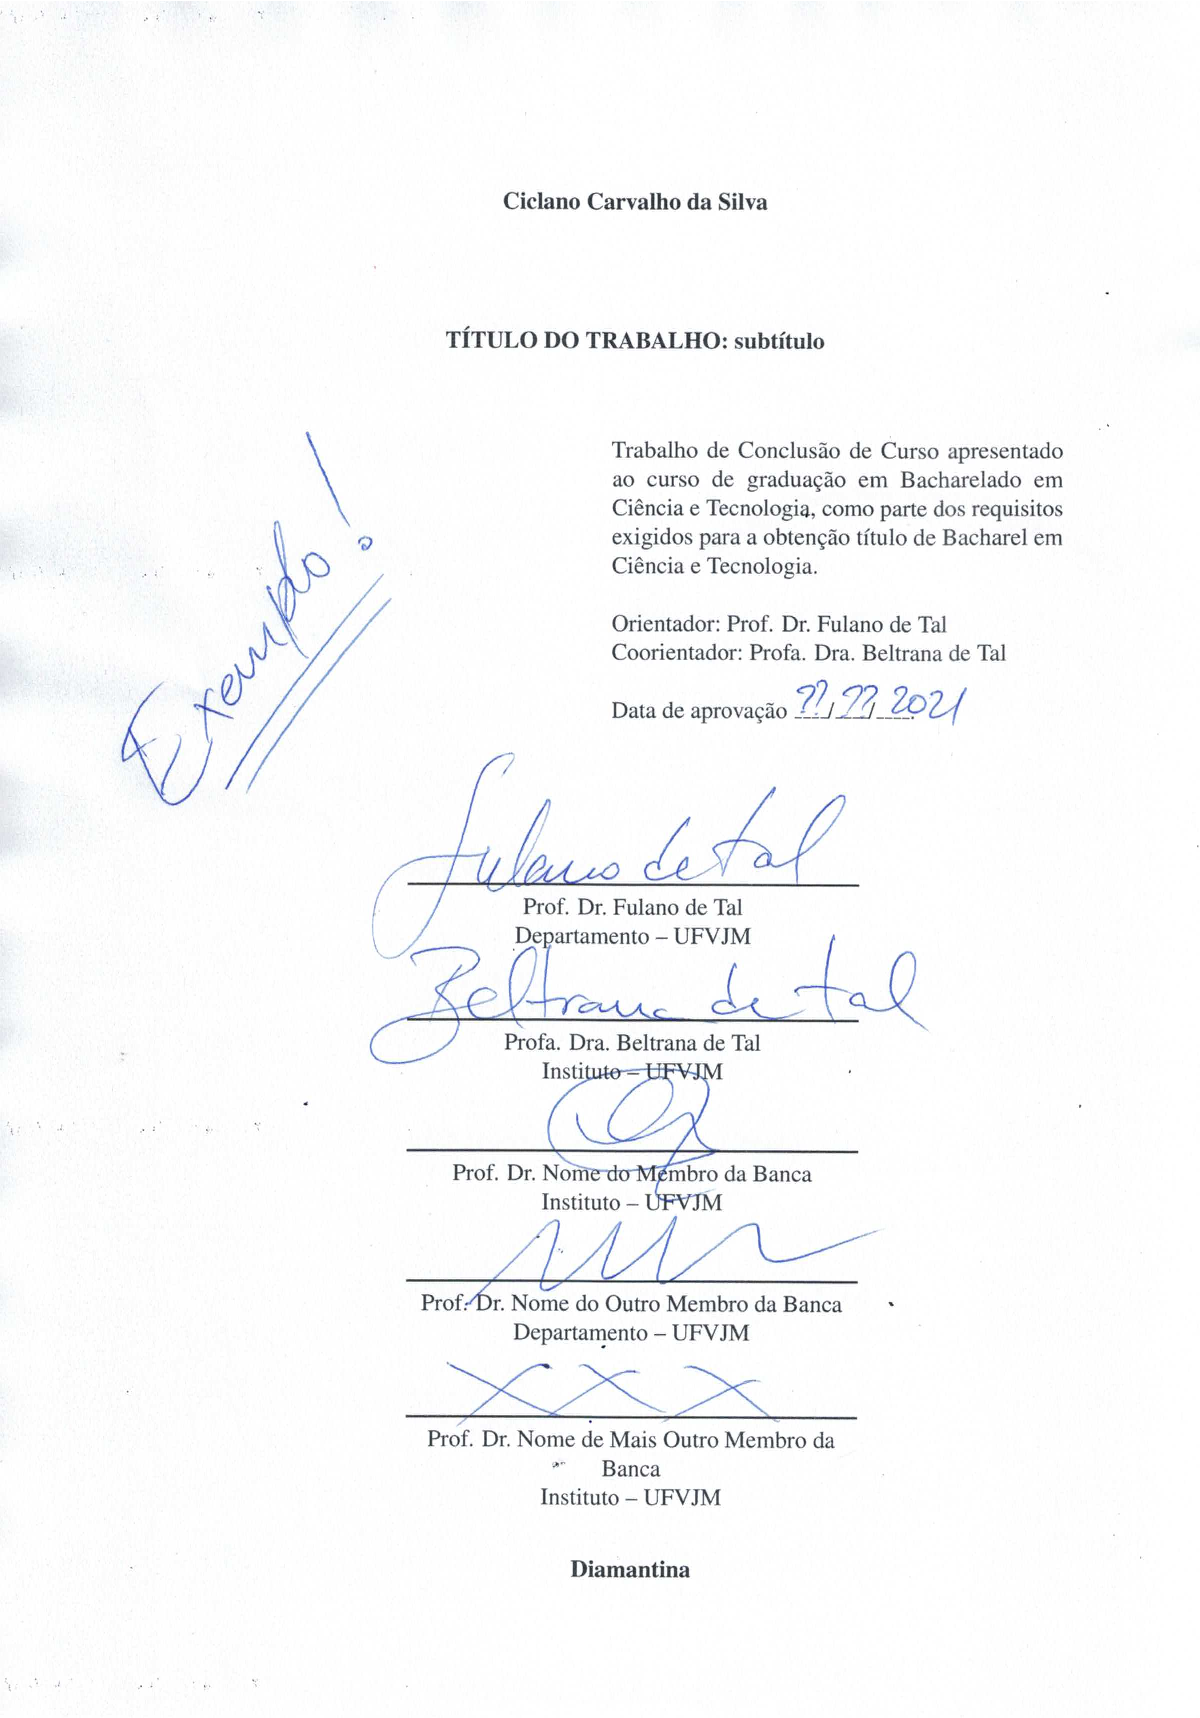
\includepdf{FolhaAprovacao.pdf}
%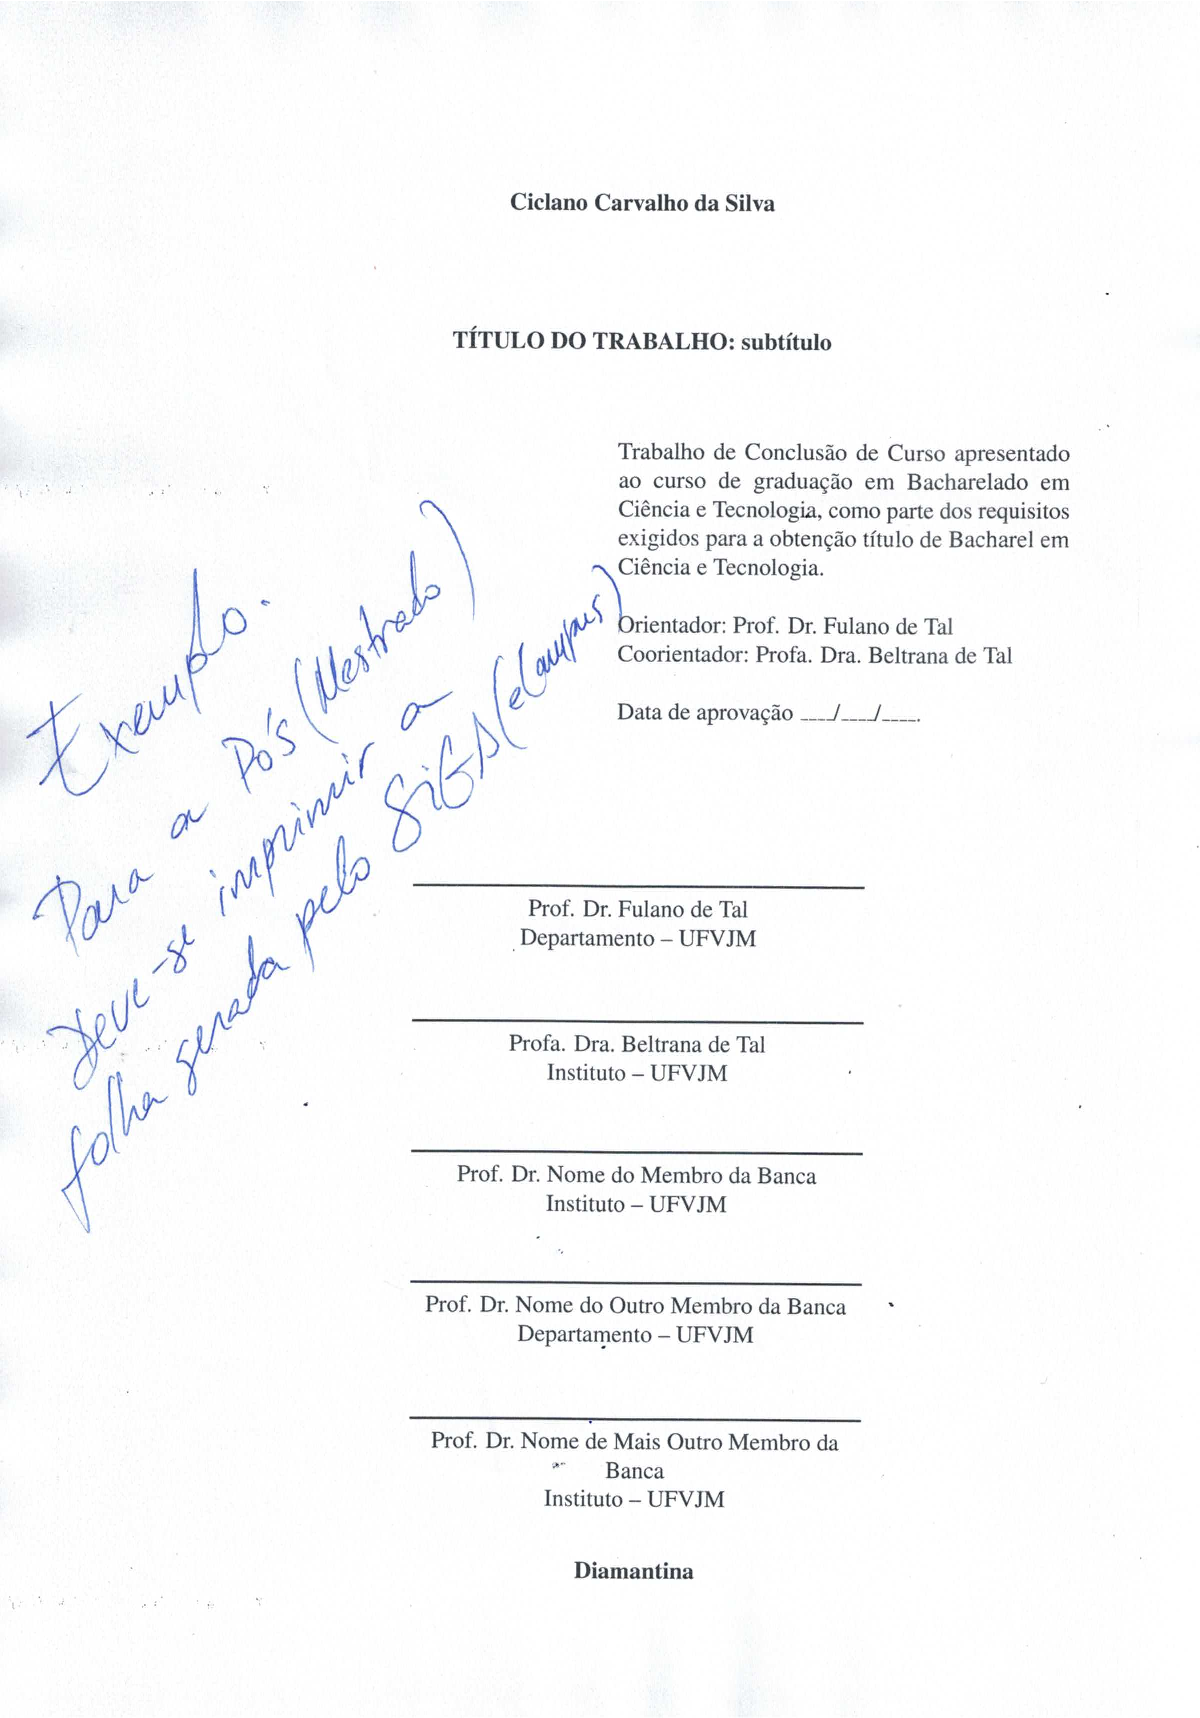
\includepdf{FolhaAprovacaoSemAssinaturas.pdf}
%==============================================

\cleardoublepage %insere página em branco depois da folha de aprovação para a impressão frente e verso

%%%%%%%%%%%%%%%%%%%%%%%%%%%%%%%%%%%%%%%%%%%%%%%%%%%%%%%%%%%%%%%%%%%
%% Dedicatória

\begin{dedicatoria}
\vspace*{\fill}
\begin{flushright}

\end{flushright}
\end{dedicatoria}
      %% Dedicatória       - opcional 
%%%%%%%%%%%%%%%%%%%%%%%%%%%%%%%%%%%%%%%%%%%%%%%%%%%%%%%%%%%%%%%%%%%
%% Agradecimentos

\begin{agradecimentos}
 
\end{agradecimentos}
   %% Agradecimentos    - opcional 
%%%%%%%%%%%%%%%%%%%%%%%%%%%%%%%%%%%%%%%%%%%%%%%%%%%%%%%%%%%%%%%%%%%
%% Epígrafe 

\begin{epigrafe}
\vspace*{\fill}
\begin{flushleft}
\justify
\hspace{4cm} 


\end{flushleft}

\end{epigrafe}
         %% Epígrafe          - opcional

\chapter*{Resumo}

\vspace{0.4cm}

\noindent 

\begin{labeling}{\textbf{Palavras-chave:}}
\item[\textbf{Palavras-chave:}] 

\end{labeling}

%%%%%%%%%%%%%%%%%%%%%%%%%%%%%%%%%%%%%%%%%%%%%%%%%%%%%%%%%%%%%%%%%%%%%%
%%% Comente o texto abaixo 
% \textcolor{red}{(as palavras-chave são separadas por ponto) (deve-se dar preferência ao uso de palavras-chave cadastradas em \url{http://acervo.bn.br/sophia_web/index.html}.)}
        %% Resumo
\chapter*{Abstract}
\vspace{4cm}
\noindent
Com as mesmas características e conteúdo do resumo em língua portuguesa, porém, deve ser escrito em língua inglesa.

\begin{labeling}{\textbf{Keywords:}}
\item[\textbf{Keywords:}] 
Word1. 
Word2. 
Word3. 
Word4. 
Word5.
\end{labeling}
      %% Abstract

%%%%%%%%%%%%%%%%%%%%%%%%%%%%%%%%%%%%%%%%%%%%%%%%%%%%%%%%%%%%%%%%%%%
%% LISTA DE FIGURAS
%%
%% A lista de figuras é gerada automaticamente
%% Esse arquivo não precisa ser modificado

\cleardoublepage

\pdfbookmark[0]{\listofalgoritmosname}{loalg}
\listofalgoritmos*
\pdfbookmark[0]{\listfigurename}{lof}
\listoffigures*
\pdfbookmark[0]{\listofgraficosname}{logrf}
\listofgraficos*
\pdfbookmark[0]{\listofmapasname}{lom}
\listofmapas*
%\pdfbookmark[0]{\listofquadrosname}{loq}
%\listofquadros*

\newpage

\cleardoublepage

% \cleardoublepage
% \pdfbookmark[0]{\listfigurename}{lof}
% \listoffigures*
% \cleardoublepage
    %% Lista de figuras  - opcional 
%%%%%%%%%%%%%%%%%%%%%%%%%%%%%%%%%%%%%%%%%%%%%%%%%%%%%%%%%%%%%%%%%%%5
%% LISTA DE TABELAS
%%
%% A lista de tabelas é gerada automaticamente
%% Esse arquivo não precisa ser modificado

\cleardoublepage
\pdfbookmark[0]{\listtablename}{lot}
\listoftables*

\newpage
    %% Lista de tabelas  - opcional 

%%%%%%%%%%%%%%%%%%%%%%%%%%%%%%%%%%%%%%%%%%%%%%%%%%%%%%%%%%%%%%%%%%%5
%% LISTA DE QUADROS
%%
%% A lista de quadros é gerada automaticamente
%% Esse arquivo não precisa ser modificado
\newpage
\cleardoublepage
\pdfbookmark[0]{\listofquadrosname}{lot}
\listofquadros*

\newpage


\newpage
%%%%%%%%%%%%%%%%%%%%%%%%%%%%%%%%%%%%%%%%%%%%%%%%%%%%%%%%%%%%%%%%%%%%
%% LISTA DE SIGLAS

\cleardoublepage
\begin{siglas}
\item [UFVJM] Universidade Federal dos Vales do Jequitinhonha e Mucuri
\item [UFMG] Universidade Federal de Minas Gerais
\item [IFNMG] Instituto Federal de Educação, Ciência e Tecnologia do Norte de Minas Gerais
\end{siglas}     %% Lista de siglas   - opcional
%%%%%%%%%%%%%%%%%%%%%%%%%%%%%%%%%%%%%%%%%%%%%%%%%%%%%%%%%%%%%%%%%%%%
%% LISTA DE SÍMBOLOS

\cleardoublepage
\begin{simbolos}
\item[$ \Gamma $] Letra grega Gama
\item[$ \Lambda $] Lambda
\item[$ \zeta $] Letra grega minúscula zeta
\item[$ \in $] Pertence
\end{simbolos}   %% Lista de símbolos - opcional

\tableofcontents*             %% Sumário

\newpage
\textual

\pagestyle{simple} %%%% Esse comando tira o cabeçalho do modelo abntex2 original.

% \input{capitulos/cap_Introducao.tex}
%\input{capitulos/introducao.tex}
%\input{capitulos/revisao-de-literatura}
% \chapter{Material e Métodos (ou Metodologia).}
\label{ch:metodologia}
%Falar porquê do Scrum
%Falar o porquê do Plone

Como você realizou seu trabalho?

\section{Primeira seção da Metodologia}

Texto da primeira seção.

\section{Segunda seção da Metodologia.}

Texto da segunda seção.

% \chapter{Discussão.}

Discuta aqui os resultados do seu trabalho\index{equação com numeração!outro teste}.
%Note que o comando \index é usado para inserir "outro teste" como subitem de "equação com numeração" no Índice.

\section{Primeira seção da Discussão.}

Texto da primeira seção.

\section{Segunda seção da Discussão.}

Texto da segunda seção.

% \chapter{Resultados.}

Quais foram os resultados que você obteve com o seu trabalho?

\section{Primeira seção dos Resultados.}

Texto da primeira seção.

\section{Segunda seção dos Resultados.}

Texto da segunda seção.

% \chapter{Considerações Finais (Opcional).}

Citar aqui trabalhos futuros e outras considerações.




% Deixar espaço em branco entre o final do trabalho e a bibliografia para evitar problemas de espaçamento entre linhas
%%%%%%%%%%%%%%%%%

%%%%%%%%%%%%%%%%%
\bibliography{bibliografia}  %% Gera as referências

\apendices
%\chapter{Apendice1}
\label{ch:apendice1}

\includepdf[pages=-]{pos-textual/Apendice1.pdf}


\anexos
%\chapter{Anexo1}
\label{ch:anexo1}

\includepdf[pages=-]{pos-textual/Anexo1.pdf}

% \chapter{Título do Anexo}

Exemplo de Anexo...

Lorem ipsum congue aliquam sollicitudin lorem donec hac libero, in nunc faucibus torquent platea porta molestie habitasse, elit senectus commodo taciti ullamcorper a vestibulum. lobortis suscipit nullam id habitant nulla sem torquent, aenean arcu sed aliquam platea aenean, nullam fringilla primis magna tellus ullamcorper. curae aptent lacinia diam tincidunt eleifend nam dapibus dictum ultricies fames bibendum mauris consectetur tristique imperdiet convallis tempus, ullamcorper torquent tempus sem dictumst aenean per libero nibh adipiscing phasellus purus dictumst sodales ad. eleifend bibendum mollis sodales egestas ac lorem tortor et nullam magna volutpat proin netus nam, luctus urna praesent sociosqu himenaeos rutrum diam cras aenean nibh vivamus interdum. 

Aliquam tristique aliquam aliquet purus ullamcorper lorem egestas suscipit vel aenean lobortis, curabitur sed faucibus volutpat ipsum nunc ante iaculis lacinia a magna, consequat fusce libero blandit semper felis nullam amet et lobortis. aliquam imperdiet tempor hendrerit sit neque venenatis, ultrices pharetra aptent primis auctor quisque aenean, libero vivamus adipiscing maecenas dui. sociosqu consequat tempus lectus torquent at ac torquent varius nunc, per interdum cubilia felis tincidunt iaculis ad laoreet donec hendrerit, velit convallis primis nunc ad habitasse maecenas sapien. ante vulputate varius ultricies cubilia viverra dolor consectetur tellus morbi, duis porta ut placerat aliquam sagittis felis faucibus, torquent suspendisse mi egestas eu ipsum volutpat conubia augue, cursus sociosqu donec quis euismod himenaeos morbi. 

Facilisis lorem tortor molestie augue nostra nam consequat, ac dictumst enim nec taciti torquent, mattis semper vulputate aenean massa fames. mollis massa molestie urna maecenas sodales mollis cursus cras, elit sagittis vivamus euismod risus diam nibh sem, diam elementum ullamcorper consequat faucibus pellentesque rhoncus. scelerisque diam donec hendrerit nam ut lacus vitae tellus nisi nullam, imperdiet turpis lorem bibendum fames inceptos congue praesent platea eros, consectetur venenatis fermentum platea aliquam senectus pharetra faucibus litora. augue consectetur amet viverra aptent ullamcorper dolor iaculis euismod curabitur in, mollis senectus lacinia commodo vestibulum malesuada aptent sagittis elit, donec aptent malesuada lacus libero rutrum morbi diam dui. 

Id sagittis at potenti elementum lacinia porttitor tristique elementum phasellus etiam est eget, justo a viverra lobortis lorem cubilia tempus scelerisque tincidunt semper. eleifend euismod blandit purus aliquam duis mi praesent quisque id, semper suspendisse mauris amet commodo nec elit ultricies velit, conubia lobortis habitasse etiam varius blandit sit bibendum. ultricies orci feugiat egestas litora accumsan bibendum proin vehicula leo vel, quam tincidunt class vel ornare est euismod eros platea duis, semper curabitur class nam non nec aptent massa nostra. class purus blandit aenean arcu convallis lectus donec habitasse tincidunt inceptos aliquam libero, nulla aliquam risus quisque sagittis nunc quis luctus tempus rhoncus. 

Scelerisque dolor lacus proin ut molestie condimentum semper condimentum, eu habitasse nam mi tempus ante scelerisque aliquam fames, suspendisse dictum commodo urna dapibus est proin. senectus adipiscing ligula suspendisse suscipit morbi nisi elit faucibus vehicula dictum rutrum taciti, habitasse himenaeos scelerisque sodales platea dictum semper vehicula ullamcorper conubia sodales, congue dolor gravida mauris lorem scelerisque nostra maecenas tristique auctor scelerisque. fames posuere litora cubilia conubia sit, quisque netus ut ligula nunc nostra, nisi tempus lorem tellus. 

%%%%%%%%%%%%%%%%%%%%%%%%%%%%%%%%%%%%%%%%%%%%%%%%%%%%%%%%%%%%%%%%%%%%%%%%%%%%%
%% Fim do documento
\end{document}
%%%%%%%%%%%%%%%%%%%%%%%%%%%%%%%%%%%%%%%%%%%%%%%%%%%%%%%%%%%%%%%%%%%%%%%%%%%%%


